\section{Juegos Matem\'aticos}

A Conway siempre le interesaron los juegos, era un jugador adicto al backgammon y de sus primeros aportes a la columna de Martin Gardner eran juegos que el hab\'ia creado, por ejemplo el juego Sprouts, creado por Conway en compa\~nia con el entonces estudiante de posgrado Mike Paterson, fue descrito en una carta que Conway le envi\'o a Gardner en 1967 y ese mismo a\~no Gardner la public\'o en su columna \cite{}.

Por eso, no es sorpresa, que al rededor del a\~no 1970, al descubrir el teorema de Sprague-Grundy, se obsesionara con los juegos. El teorema de Sprague-Grundy\cite{}, es un teorema que trata sobre los juegos imparciales, estos son aquellos juegos de informaci\'on perfecta, sin azar, tales que los movimientos posibles dependan solamente del tablero y no de qu\'e jugador est\'e jugando.

Vamos a explicar esta definici\'on parte por parte. Un juego de informaci\'on perfecta es un juego donde cada persona sabe cu\'ales movimientos pueden hacer los otros jugadores, en este sentido juegos como el p\'oker o el black-jack quedan descartados, puesto que los jugadores no saben qu\'e cartas tienen los otros. Un juego sin azar es un juego donde los movimientos no dependen del azar, no hay ning\'un dado que dicte los movimientos ni hay nig\'un generador de n\'umeros aleatorios que dicte el ganador, en este caso quedan descartados juegos como el parqu\'es, parch\'is o como la loter\'ia. La \'ultima condici\'on es la que le da el nombre de imparciales, esta es, si tenemos la posici\'on del tablero los movimientos posibles para los jugadores son los mismos, aqu\'i se descartan la mayor\'ia de otros juegos que se conocen, por ejemplo, el ajedrez tiene diferentes movimientos para los dos jugadores, uno juega con las fichas blancas y el otro con las fichas negras, o por ejemplo el triqui (tic-tac-toe), en este un jugador juega con las cruces (`X') y otro con los c\'irculos (`O'). F\'ijese en las figuras \ref{figure:game-chess} y \ref{figure:game-triqui}, en ambos tableros los posibles movimientos para las fichas negras y para las fichas blancas son diferentes, si le tocara jugar a un jugador ser\'ia este podr\'ia ganar, mientras que si le toca jugar al otro jugador este no tendr\'ia la posibilidad de ganar en ese movimiento.

\TwoFig{images/games-partisan-1.png} % image 1
         {Tablero de ajedrez donde el jugador con las fichas negras puede ganar en un movimiento, pero el jugador con las blancas no. \textit{(Fuente: lichess.com)}} % caption 1
         {figure:game-chess} % label 1
         {images/games-partisan-2.png} % image 2
         {Tablero de triqui donde el jugador con las `X' puede ganar en un movimiento, pero el jugador con las `O' no. \textit{(Google)}} % caption 2
         {figure:game-triqui} % label 2

Un ejemplo de juego al que s\'i se le puede aplicar el teorema de Sprague-Grundy, es decir un juego imparcial, es el comunmente juego 21. En el juego se van turnando entre dos personas, el primer jugador dice el n\'umero `1' y el siguiente jugador tiene que aumentar el n\'umero en `1', `2' o `3'. Pierde el jugador que diga `21' o un n\'umero mayor que `21'. Un ejemplo de c\'omo un juego de `21' puede pasar es:

\begin{center}
    \begin{tabular}{|c|M{3cm}|}
        \hline
        Jugador & \text{N\'umero} \\
        \hline\hline
        1 & 1 \\
        \hline
        2 & 4 \\
        \hline
        1 & 7 \\
        \hline
        2 & 10 \\
        \hline
        1 & 11 \\
        \hline
        2 & 13 \\
        \hline
        1 & 16 \\
        \hline
        2 & 17 \\
        \hline
        1 & 20 \\
        \hline
        2 & 21 \\
        \hline
    \end{tabular}
\end{center}

Ac\'a el jugador 1 gan\'o porque el jugador 2 dijo 21. F\'ijese que en este juego las opciones para los dos jugadores son las mismas, el `tablero' de este juego consistir\'ia en el n\'umero que se ha dicho inmediatamente en el turno anterior.

El teorema de Sprague-Grundy le asigna un valor a todos los juegos de este tipo con el que se puede calcular qu\'e jugador va a ganar (jugando de la mejor manera), si el primero o el segundo. Adem\'as de todo, el teorema da una forma en la que se pueden calcular valores de juegos que consisten en la combinaci\'on de otros juegos m\'as simples, por ejemplo, si quisieramos jugar dos juegos imparciales al mismo tiempo pero en cada turno solo podr\'iamos hacer un movimiento en uno de los dos juegos, el teorema de Sprague-Grundy nos dir\'ia como calcular qui\'en ganar\'ia con base a los valores de cada uno de los juegos imparciales.

Conway quer\'ia generalizar este teorema pero para juegos m\'as generales, los llamados juegos partisanos. Los juegos partisanos son tambi\'en juegos sin azar y de informaci\'on perfecta, pero en este caso no tenemos la condici\'on extra de imparcialidad, entonces entran juegos como el ajedrez, el triqui o el go.

En la \'epoca de 1970 sucedieron var\'ias cosas que ayudaron al estudio de estos juegos. Primero, Jon Diamond, el campe\'on brit\'anico de Go durante 11 a\~nos \cite{}(https://www.britgo.org/people/diamondj), entr\'o a estudiar matem\'aticas en Cambridge. \'El fund\'o la \textit{Cambdridge Go Society} y con eso incentiv\'o el juego dentro de Cambridge.
Conway se interes\'o por el Go principalmente porque los juegos de Go tienen la propiedad de que casi al final de la partida, el tablero se separa en ciertas zonas, casi como si se estuvieran jugando varios juegos simultaneamente, cada jugador eligiendo en cada turno en qu\'e parte jugar.

La otra cosa que ayud\'o al desarrollo de la teor\'ia fue el inter\'es de Richard Guy y Elwyn Berlekamp en los juegos. Elwyn Berlekamp fue un matem\'atico y cient\'ifico de la computaci\'on que ya hab\'ia trabajado en juegos antes, su tesis de maestr\'ia hab\'ia sido en algoritmos para resolver problemas del bridge (el juego de cartas), y mientras trabajaba en Bell Labs hizo un reporte t\'ecino del juego de cuadritos, un juego a lapiz y papel donde los jugadores se turnan conectando puntos adyacentes en una cuadr\'icula y gana el que haya hecho m\'as cuadritos. Richard Guy, el mismo que descubri\'o el \textit{glider} del juego de la vida, conoc\'ia a los dos y fue el puente para que los tres trabajaran juntos.

Los tres dieron vida a \textit{Winning Ways for Your Mathematical Plays}, un compendio de cuatro volumenes con toda la informaci\'on que ten\'ian sobre juegos matem\'aticos. Un trabajo que se demor\'o quince a\~nos en salir a la luz, con dos volumenes, y luego en una segunda edici\'on 20 a\~nos despu\'es con dos volumenes m\'as.

En este compendi\'o desarrollaron la teor\'ia de los juegos partisanos y la extendieron. En los libros aplican la teor\'ia a much\'isimos juegos diversos, tanto a juegos imparciales como a juegos partisanos, y extienden el teorema de Sprague-Grundy a juegos partisanos tambi\'en.

\subsection{Hackenbush}

Un juego que nos permite explicar una parte de la teor\'ia de manera m\'as directa es el juego del Hackenbush. El juego lo invent\'o Conway pero el nombre del juego fue creado por Richard Guy inspirado en un personaje de la pel\'icula de 1937 \textit{A Day at the Races}, le puso as\'i porque el juego consiste en cortar (\textit{hack} en ingl\'es) arbustos (\textit{bushes} en ingl\'es).

\begin{figure}[h]
    \centering
    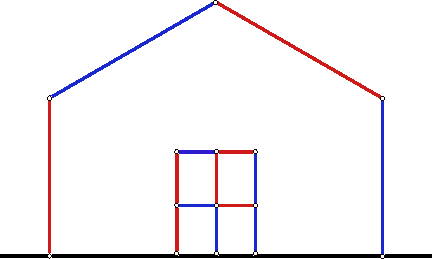
\includegraphics[width=.7\textwidth]{images/hackenbush-first_example.pdf}
    \caption{Una posible configuraci\'on inicial del juego del Hackenbush.}
\end{figure}

El juego empieza con una configuraci\'on de l\'ineas, unas rojas y otras azules. Todas las l\'ineas tienen que estar conectadas al piso, ya sea directamente, o a trav\'es de otras que s\'i lo est\'en. El juego se juega por turnos, cada uno de los jugadores tiene un color asignado, el primer jugador juega con las azules y el segundo juega con las rojas. En cada turno el jugador tiene que borrar una l\'inea de su color, y si alguna de las otras l\'ineas queda desconectada entonces esa tambi\'en se borra. Es como si se estuvieran cortando arbustos, si se corta el tallo del arbusto entonces este se va a caer al piso y ya no va a estar en el juego.


\begin{figure}[h]
    \centering
    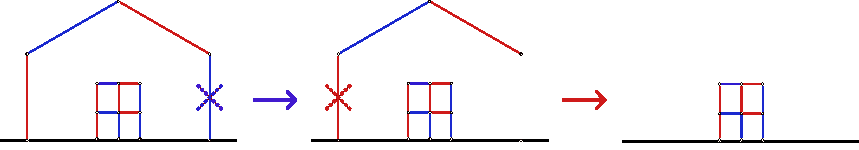
\includegraphics[width=.7\textwidth]{images/hackenbush-game_example.pdf}
    \caption{Jugando Hackenbush.}
\end{figure}


Lo interesante del juego es que tiene esta propiedad que estaba buscando Conway en juegos partisanos, algunas configuraciones tienen ciertos `arbustos' desconectados, por lo tanto cada uno de estos arbustos se puede tratar como un juego separado, as\'i como lo muestra la im\'agen de la figura \ref{figure:hackenbush_sum}. El hackenbush lo vamos a utilizar en lo que queda de esta secci\'on para mostrar como se calculan los valores de un juego en general, para todos los juegos se puede hacer una construcci\'on parecida pero otros juegos tienen particularidades espec\'ificas que puede que aplicar la teor\'ia sea m\'as dificil. Lo bueno del hackenbush, es que es casi que un juego diseñado para que ilustrar la teor\'ia sea m\'as sencillo.

\begin{figure}[h]
    \centering
    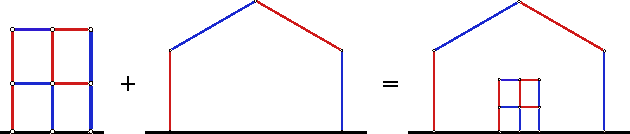
\includegraphics[width=.7\textwidth]{images/hackenbush-sum_example.pdf}
    \caption{La puerta y el contorno de la casa se pueden tomar como juegos separados.}
    \label{figure:hackenbush_sum}
\end{figure}


\subsection{Valores de juegos}

Para un estado del juego, en este caso el hackenbush, tenemos los posibles movimientos que puede hacer el jugador de las l\'ineas azules y los posibles movimientos que puede hacer el jugador de las l\'ineas azules. Si calculamos los valores para esos estados antes, vamos a calcular el valor de nuestro estado con respecto a esos posibles estados siguientes.

Sea $L$ el conjunto de los valores de los estados a los que puede llegar el jugador azul, y sea $R$ el del jugador rojo, entonces el valor de nuestro estado se va a definir como $\surr{L}{R}$. En la figura \ref{figure:hackenbush_val} podemos ver un ejemplo de esto, si bien en la figura se muestra los estados siguientes la idea es guardar solamente los valores.

\begin{figure}[h]
    \centering
    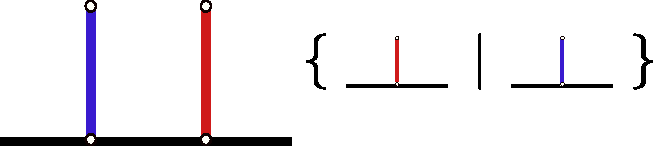
\includegraphics[width=.7\textwidth]{images/hackenbush-val_example.pdf}
    \caption{A la izquierda el estado del juego, y a la derecha sus movimientos.}
    \label{figure:hackenbush_val}
\end{figure}

En cierto sentido, los valores est\'an definidos a partir de los valores siguientes, y estos valores siguientes est\'an definidos a partir de los siguientes, y as\'i hasta que se acabe el juego. El hackenbush termina cuando no hay ninguna l\'inea en el estado, por lo tanto vamos a tomar este como nuestro caso base, a ese estado le asignaremos un valor de $0$. 

En general cuando analizamos un juego es mejor empezar desde sus \'ultimos movimientos, sus movimientos m\'as b\'asicos, para ver c\'omo se puede ganar. En el caso del hackenbush los siguientes movimientos m\'as b\'asicos son cuando existe solo una l\'inea, sea roja o azul. Si la l\'inea es azul entonces el valor es $\surr{0}{}$, mientras que si la l\'inea es roja el valor es $\surr{}{0}$, a estos valores los llamaremos $1$ y $-1$ respectivamente, as\'i como lo indica la figura \ref{figure:hackenbush_roots}.

\begin{figure}[h]
    \centering
    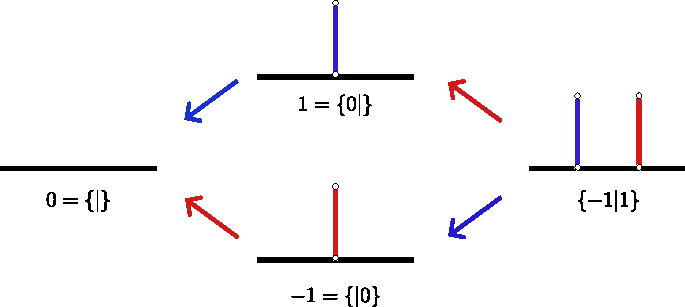
\includegraphics[width=.7\textwidth]{images/hackenbush-surr_roots.pdf}
    \caption{Diagrama de los casos base. Cada flecha indica un movimiento, y el color corresponde al jugador que lo hace.}
    \label{figure:hackenbush_roots}
\end{figure}

Lo que intentan capturar estos valores es el sesgo que tiene el tablero para un jugador o el otro, los tableros con valores mayores positivos van a ser ganados por el jugador azul y los de valores negativos van a ser ganados por el jugador rojo. Pero hay otro tipo de tableros, aquellos que no tienen ning\'un sesgo de color, como el de la derecha de la figura \ref{figure:hackenbush_roots}. En este tablero gana el jugador que juegue de segundas, si empieza el azul gana el rojo, y si empieza el rojo gana el azul, en estos tableros el valor va a ser igual a $0$, por lo tanto tenemos que $0=\surr{-1}{1}$.

Esta definici\'on de $0=\surr{-1}{1}$ es consistente con lo que hab\'iamos dicho de sumar los juegos. Otra forma de verificar el valor de este juego es darse cuenta que este juego equivale a la suma de dos juegos, el de la izquierda es solo una l\'inea azul, y el de la derecha es solo una l\'inea roja, estos juegos valen respectivamente $1$ y $-1$, por lo tanto el valor del juego va a ser igual al valor de su suma, $1+(-1) = 0$.

En la secci\'on \ref{section:surreal} de n\'umeros surreales nos acercamos a esta definici\'on desde otro \'ambito.

\subsection{Comparando juegos}

Ya teniendo un juego de valor $1$, y otro juego de valor $-1$, podemos crear juegos de valores $n$ y de valores $-n$ para todos los $n$ n\'umeros naturales. Estos ser\'ian $n$ l\'ineas de color azul para el caso de un juego de valor $n$, y $n$ l\'ineas de color rojo para un juego de valor $-n$. Con estos ya podemos intentar calcular los valores de otros juegos m\'as complejos.

\begin{figure}[b]
    \centering
    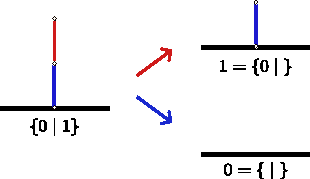
\includegraphics[width=.5\textwidth]{images/hackenbush-half_def.pdf}
    \caption{El valor del diagrama calculado.}
    \label{figure:hackenbush-half}
\end{figure}


Hagamos un ejemplo, consideremos dos l\'ineas pegadas verticalmente, la de abajo azul y la de arriba rojo, exactamente como en la figura \ref{figure:hackenbush-half}. Si jugamos la posici\'on nos damos cuenta que el valor es positivo, ya que el azul siempre va a ganar, pero, ¿Exactamente cu\'anto es el valor?

Algo que nos podemos poner a hacer es compararlo con juegos de valor $-n$, si al sumarlo con el juego todav\'ia sigue ganando el azul esto significa que el valor del juego es menor que $n$. Haciendo esto podemos ver que el valor de nuestro juego est\'a entre $0$ y $1$, esto es, si le sumamos un juego de una l\'inea roja al nuestro entonces gana el rojo. En otras palabras, $0 < \surr{0}{1} < 1$. Lo interesante de $\surr{0}{1}$ es que entonces no es un valor entero, por lo tanto lo siguiente que tendremos que hacer es ver entre qu\'e valores racionales est\'a.

Para esto, lo primero que hacemos es sumar dos veces este juego y compararlo con un juego de valor $-1$, es decir, con un juego de una l\'inea roja, nuestro juego quedar\'ia como en la parte izquierda de la figura \ref{figure:hackenbush-half_proof}. Si en este juego gana el jugador rojo eso significa que dos veces el valor del juego es menor que $1$, si gana el jugador azul significa que es mayor que $1$, y si gana el segundo jugador esto significa que el valor es precisamente $\frac{1}{2}$ ya que dos veces el juego es exactamente $1$.

\begin{figure}[h]
    \centering
    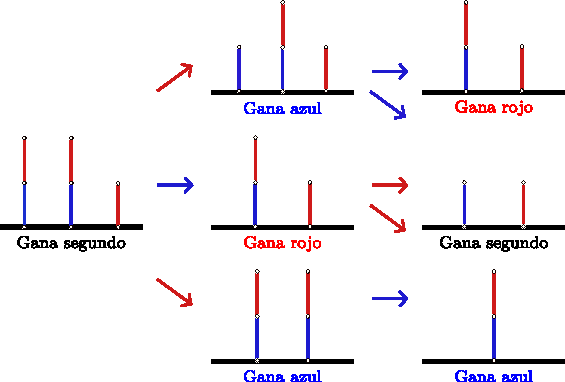
\includegraphics[width=.7\textwidth]{images/hackenbush-half_proof.pdf}
    \caption{Demostraci\'on gr\'afica de que $\surr{0}{1}=\frac{1}{2}$.}
    \label{figure:hackenbush-half_proof}
\end{figure}

Lo interesante de este an\'alisis es que con argumentos parecidos podemos calcular el valor de cualquier juego de Hackenbush, y, sabiendo propiedades de estos valores, como las demostradas en la secci\'on \ref{section:surreal}, podemos hacer este c\'alculo incluso m\'as r\'apido.

Por ejemplo, una propiedad es que si el valor es $x=\surr{L}{R}$, entonces se puede mostrar que $x$ es mayor que todos los elementos de $L$ y menor que todos los elementos de $R$. Por lo tanto, si un elemento de $L$ es positivo o $0$, entonces $x$ es positivo, por lo tanto gana el azul. Esto se traducir\'ia a los juegos como, si el jugador azul puede llevar el juego a un estado donde sabemos que o gana el azul o gana el segundo jugador, entonces en ese estado gana el azul.

Estos valores, llamados n\'umeros surreales, se alimentan mutuamente del lenguaje de los juegos, esto es, propiedades de los juegos muestran propiedades en los n\'umeros surreales y propiedades en los n\'umeros pueden a su vez mostrar propiedades en los juegos.